\begin{figure}[H]
  \centering
  % W=3.2, H=1.8, gap=0.7 → offsets: 0, 3.9, 7.8, 11.7
  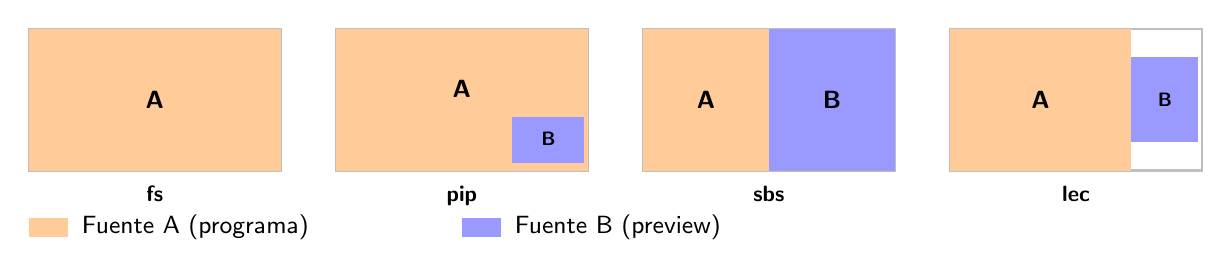
\begin{tikzpicture}[font=\sffamily\small]

    % ─────────── Full Screen (ox=0) ────────────────────────────────────
    \draw[thick, gray!50] (0,0) rectangle (3.2,1.8);
    \fill[orange!40] (0,0) rectangle (3.2,1.8);
    \node[font=\sffamily\bfseries\small] at (1.6,0.9) {A};
    \node[font=\sffamily\footnotesize, below=2pt] at (1.6,0) {\textbf{fs}};

    % ─────────── Picture in Picture (ox=3.9) ───────────────────────────
    \draw[thick, gray!50] (3.9,0) rectangle (7.1,1.8);
    \fill[orange!40] (3.9,0) rectangle (7.1,1.8);
    \node[font=\sffamily\bfseries\small] at (5.5,1.04) {A};
    \fill[blue!40] (6.14,0.10) rectangle (7.05,0.684);
    \node[font=\sffamily\bfseries\scriptsize] at (6.60,0.40) {B};
    \node[font=\sffamily\footnotesize, below=2pt] at (5.5,0) {\textbf{pip}};

    % ─────────── Side by Side (ox=7.8) ─────────────────────────────────
    \draw[thick, gray!50] (7.8,0) rectangle (11.0,1.8);
    \fill[orange!40] (7.8,0) rectangle (9.4,1.8);
    \fill[blue!40]   (9.4,0) rectangle (11.0,1.8);
    \node[font=\sffamily\bfseries\small] at (8.6,0.9) {A};
    \node[font=\sffamily\bfseries\small] at (10.2,0.9) {B};
    \node[font=\sffamily\footnotesize, below=2pt] at (9.4,0) {\textbf{sbs}};

    % ─────────── Lecture (ox=11.7) ─────────────────────────────────────
    \draw[thick, gray!50] (11.7,0) rectangle (14.9,1.8);
    \fill[orange!40] (11.7,0) rectangle (14.004,1.8);
    \fill[blue!40]   (14.004,0.36) rectangle (14.85,1.44);
    \node[font=\sffamily\bfseries\small] at (12.85,0.9) {A};
    \node[font=\sffamily\bfseries\scriptsize] at (14.43,0.9) {B};
    \node[font=\sffamily\footnotesize, below=2pt] at (13.3,0) {\textbf{lec}};

    % ─────────── leyenda ───────────────────────────────────────────────
    \fill[orange!40] (0,-0.85) rectangle (0.5,-0.60);
    \node[right, font=\sffamily\small] at (0.55,-0.72) {Fuente A (programa)};
    \fill[blue!40] (5.5,-0.85) rectangle (6.0,-0.60);
    \node[right, font=\sffamily\small] at (6.05,-0.72) {Fuente B (preview)};
  \end{tikzpicture}
  \caption{Disposición visual de las fuentes A y B en los cuatro composites
           principales de Voctomix~2.0: pantalla completa (\texttt{fs}),
           imagen en imagen (\texttt{pip}), lado a lado (\texttt{sbs}) y
           conferencia (\texttt{lec}).}
  \label{fig:composites_diagrama}
\end{figure}